\hypertarget{IU01}{\subsection{IU01 Página de inicio}}


    \subsubsection{Pantalla de bienvenida}

    Primera sección de la pantalla de inicio.
    Se encuentra el título del sistema, los nombres de los autores y la barra de navegación.

    \begin{figure}[H]
		\begin{center}
			
\includegraphics[scale=0.3]{pantallas/Index1}
			\caption{IU01/01 - Pantalla de bienvenida}
		\end{center}
	\end{figure}


    \subsubsection{Pantalla de selección de empresas}

    Para efectuar un análisis, desplácese hacia abajo para ver las empresas listadas.
    Incluya una empresa al análisis presionando sobre su el cuadro de selección a la izquierda de su nombre;
    en él aparecerá una marca, indicando que se considerará en el análisis,
    para eliminar una empresa seleccionada del análisis,
    presionar nuevamente sobre el cuadro a la izquierda,
    la marca desaparecerá.
    ``Seleccionar todo'' marca todos los cuadros y ``Limpiar'' limpia la selección.

    \begin{figure}[H]
		\begin{center}
			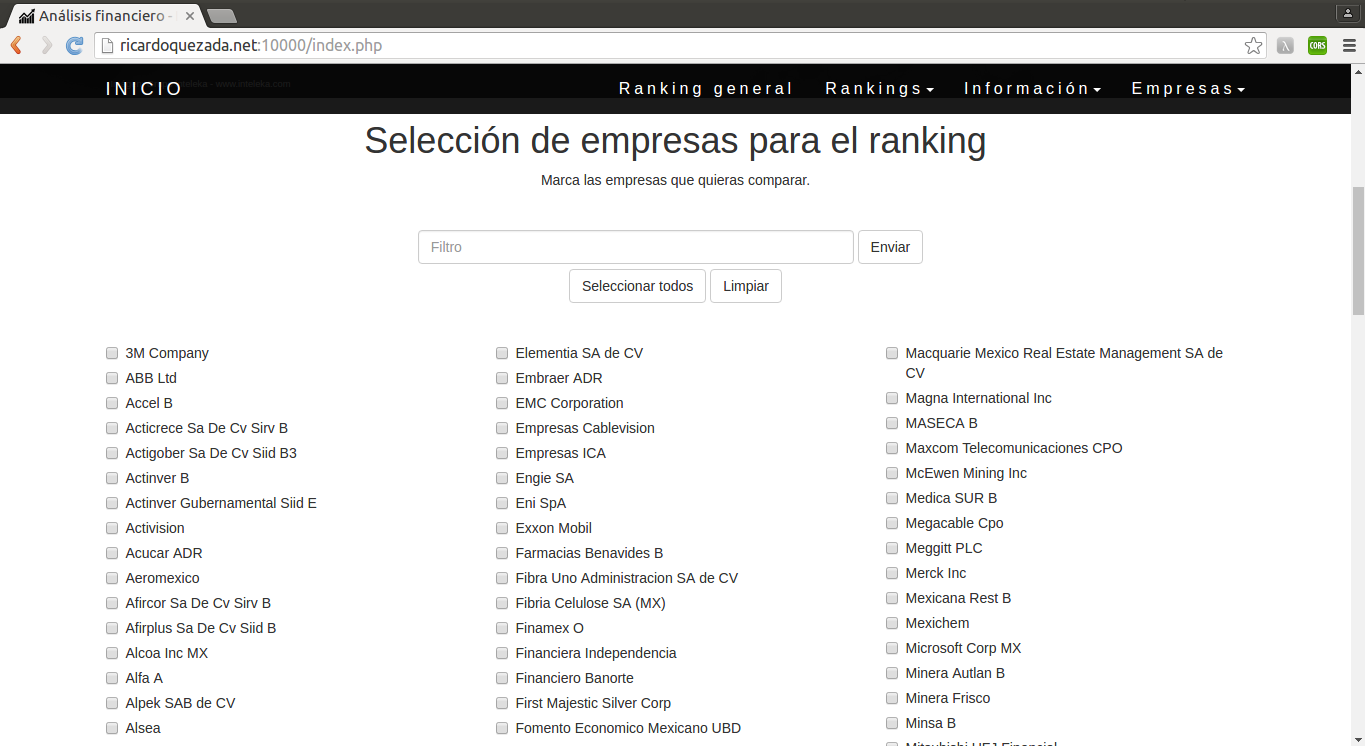
\includegraphics[scale=0.3]{pantallas/Index2}
			\caption{IU01/02 - Pantalla de selección de empresas}
		\end{center}
	\end{figure}


    \subsubsection{Funcionalidad de filtro}

    Introduzca en la barra de búsqueda el nombre de una empresa para encontrarla rápidamente,
    las opciones se reducirán a medida que escribe;
    marque la casilla a su izquierda para agregarla al análisis.

    \begin{figure}[H]
		\begin{center}
			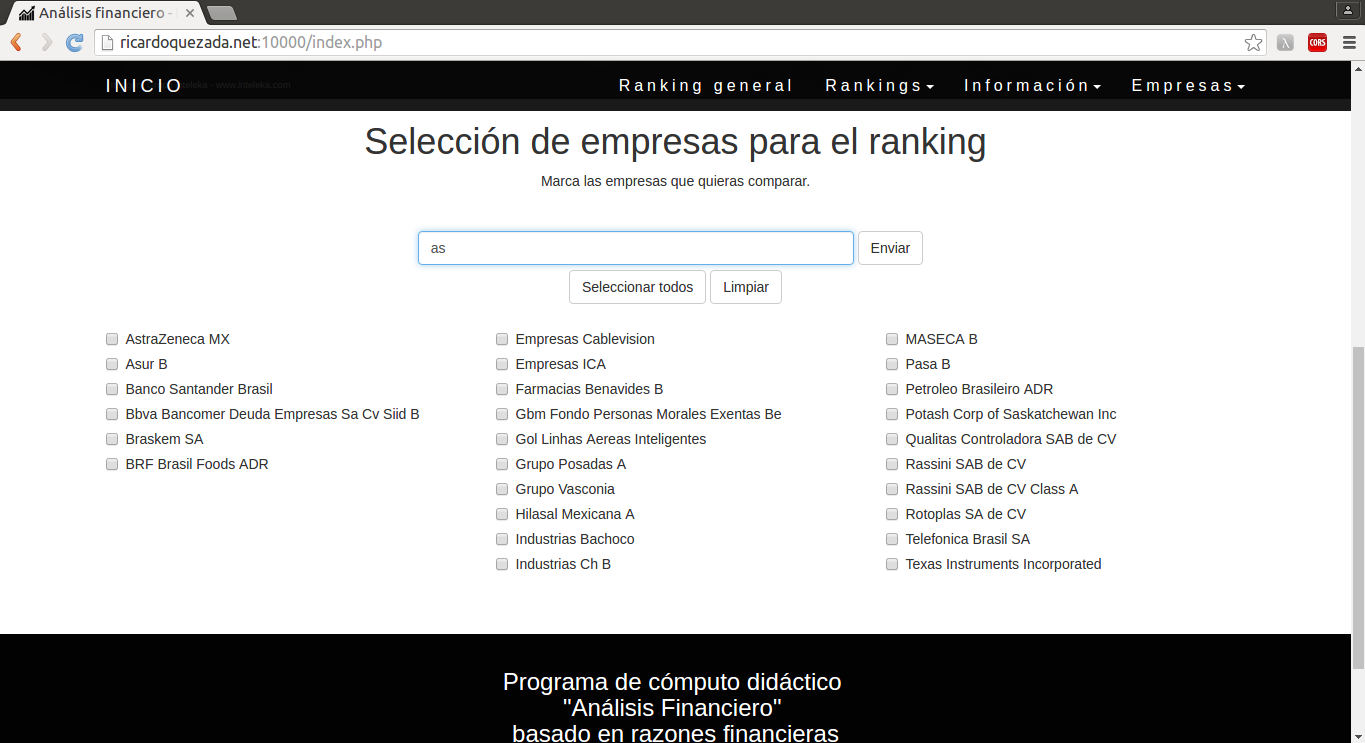
\includegraphics[scale=0.3]{pantallas/Index3}
			\caption{IU01/03 - Funcionalidad de filtro}
		\end{center}
	\end{figure}


    \subsubsection{Pantalla de envío}

    Cuando ya se han seleccionado todas las empresas a considerar,
    presione el botón ``Enviar''.
    La página comenzará a obtener la información.

    Una vez obtenida la información, se redireccióna a la página
    de ranking general.

    \begin{figure}[H]
		\begin{center}
			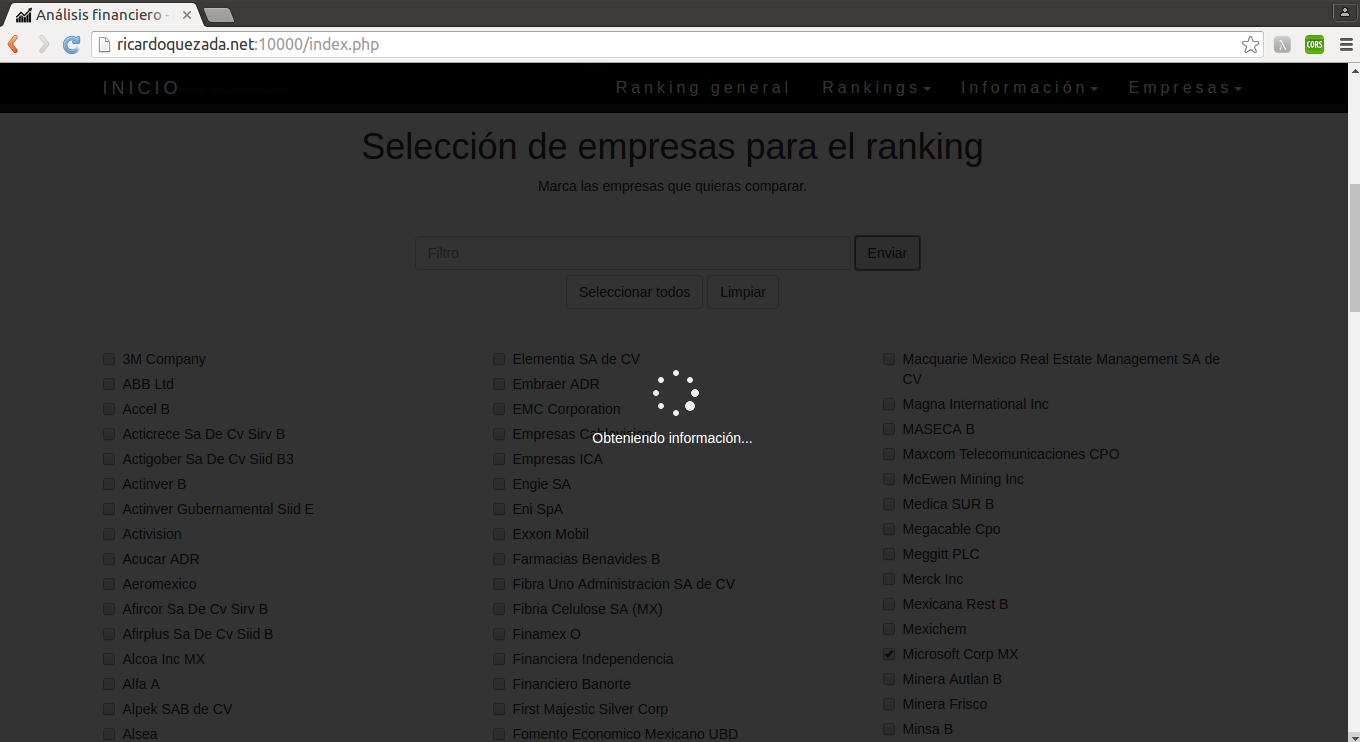
\includegraphics[scale=0.3]{pantallas/Index4}
			\caption{IU01/04 - Funcionalidad de filtro}
		\end{center}
	\end{figure}
